\documentclass[border=5mm]{standalone}
\usepackage[utf8]{inputenc}
\usepackage[T1]{fontenc}
\usepackage{amsmath}
\usepackage{tikz}
\usepackage{pgfplots}
\pgfplotsset{compat=1.18}
\usetikzlibrary{arrows.meta}
\definecolor{utnblue}{RGB}{0, 51, 102}
\definecolor{utnred}{RGB}{204, 0, 0}

% Convolución del Ej. 6a:
%   x(t) = e^{-3t} u(t)              (entrada)
%   h(t) = e^{-t/2} u(t)             (respuesta al impulso)
%   y(t) = 2/5 (e^{-t/2} - e^{-3t}) u(t)
% Paneles separados por escala: entradas (0..1) arriba, salida (0..0.4) abajo.

\begin{document}
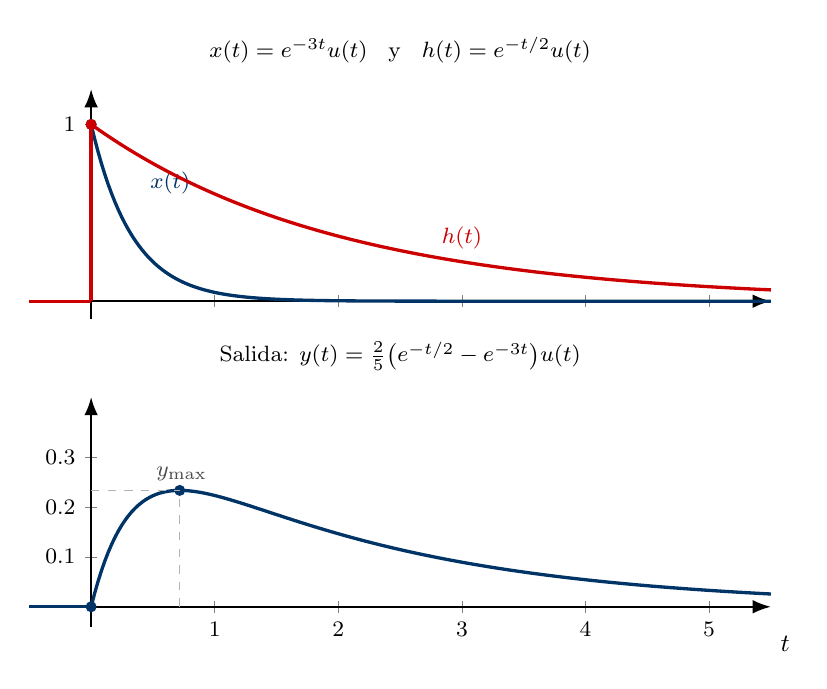
\begin{tikzpicture}[>=Latex, font=\small]

\colorlet{xcol}{utnblue}
\colorlet{hcol}{red!80!black}

\pgfmathsetmacro{\tmin}{-0.5}
\pgfmathsetmacro{\tmax}{5.5}

% =====================================================================
% PANEL SUPERIOR: entradas x(t) y h(t)
% =====================================================================
\begin{axis}[
    name=panTop,
    width=11cm, height=4.5cm,
    axis lines=center,
    xlabel={},
    ylabel={},
    xmin=\tmin, xmax=\tmax,
    ymin=-0.1, ymax=1.2,
    clip=false,
    axis line style={->, thick},
    xtick={0,1,2,3,4,5},
    xticklabels={},
    ytick={0,1},
    every tick label/.style={font=\footnotesize},
    title={\footnotesize $x(t)=e^{-3t}u(t)$\;\; y\;\; $h(t)=e^{-t/2}u(t)$},
]
    % x(t) = e^{-3t} u(t)
    \addplot[xcol, very thick, domain=\tmin:0, samples=2] {0};
    \addplot[xcol, very thick, domain=0:\tmax, samples=200] {exp(-3*x)};
    \draw[xcol, very thick] (axis cs:0,0) -- (axis cs:0,1);
    \fill[xcol] (axis cs:0,1) circle (2pt);
    \node[xcol, font=\footnotesize, above right] at (axis cs:0.4,0.55) {$x(t)$};

    % h(t) = e^{-t/2} u(t)
    \addplot[hcol, very thick, domain=\tmin:0, samples=2] {0};
    \addplot[hcol, very thick, domain=0:\tmax, samples=200] {exp(-x/2)};
    \draw[hcol, very thick] (axis cs:0,0) -- (axis cs:0,1);
    \fill[hcol] (axis cs:0,1) circle (2pt);
    \node[hcol, font=\footnotesize] at (axis cs:3.0,0.36) {$h(t)$};
\end{axis}

% =====================================================================
% PANEL INFERIOR: salida y(t)
% =====================================================================
\begin{axis}[
    name=panBot,
    at={(panTop.below south)}, anchor=north, yshift=-0.9cm,
    width=11cm, height=4.5cm,
    axis lines=center,
    xlabel={$t$},
    ylabel={},
    xlabel style={anchor=north west, at={(axis description cs:1,0)}},
    xmin=\tmin, xmax=\tmax,
    ymin=-0.04, ymax=0.42,
    clip=false,
    axis line style={->, thick},
    xtick={0,1,2,3,4,5},
    ytick={0, 0.1, 0.2, 0.3},
    every tick label/.style={font=\footnotesize},
    title={\footnotesize Salida: $y(t)=\tfrac{2}{5}\bigl(e^{-t/2}-e^{-3t}\bigr)u(t)$},
]
    % y(t) = 0 para t < 0
    \addplot[utnblue, very thick, domain=\tmin:0, samples=2] {0};
    % y(t) para t >= 0
    \addplot[utnblue, very thick, domain=0:\tmax, samples=200]
        {2/5*(exp(-x/2) - exp(-3*x))};
    \fill[utnblue] (axis cs:0, 0) circle (2pt);

    % Marcador del máximo: t* = ln(6)/2.5, y* = 2/5*(exp(-t*/2)-exp(-3t*))
    \pgfmathsetmacro{\tstar}{ln(6)/2.5}
    \pgfmathsetmacro{\ystar}{2/5*(exp(-\tstar/2) - exp(-3*\tstar))}
    \fill[utnblue] (axis cs:\tstar, \ystar) circle (2pt);
    \draw[dashed, gray!60, thin] (axis cs:\tstar, 0) -- (axis cs:\tstar, \ystar);
    \draw[dashed, gray!60, thin] (axis cs:0, \ystar) -- (axis cs:\tstar, \ystar);
    \node[font=\footnotesize, gray!60!black, anchor=south]
        at (axis cs:\tstar, \ystar) {\,$y_{\max}$};
\end{axis}

\end{tikzpicture}
\end{document}
